Бу Денгклек владеет рыбной фермой.
Рыбная ферма представляет собой водоём, который имеет вид сетки из клеток размером $N \times N$.
Каждая клетка сетки является единичным квадратом.
Столбцы сетки пронумерованы от $0$ до $N - 1$ с запада на восток, строки пронумерованы от $0$ до $N - 1$ с юга на север. 
Будем обозначать клетку, расположенную в столбце $c$ и строке $r$ сетки ($0 \le c \le N - 1$, $0 \le r \le N - 1$), как $(c, r)$.

В водоёме есть $M$ сомов, пронумерованных от $0$ до $M - 1$, расположенные в  \textbf{различных} клетках.
Для каждого $i$, для которого $0 \le i \le M - 1$, сом $i$ расположен в клетке $(X[i], Y[i])$ и весит $W[i]$ грамм.

Бу Денгклек желает построить некоторое количество пирсов для ловли рыбы.
Пирс в столбце $c$ длины $k$ (для каких-либо $0 \le c \le N - 1$ и $1 \le k \le N$) является прямоугольником, покрывающим клетки $(c, 0), (c, 1), \ldots, (c, k - 1)$.
Для каждого столбца Бу Денгклек может выбрать, строить ли в нём пирс какой-либо длины или не строить. 

Сом $i$ (при $0 \le i \le M - 1$) может быть пойман, если есть пирс, расположенный непосредственно к западу или востоку от него, и никакой пирс не покрывает его клетку, то есть
\begin{itemize}
    \item  \textbf{хотя бы одна} из клеток $(X[i] - 1, Y[i])$ или $(X[i] + 1, Y[i])$ покрыта пирсом, и
    \item нет пирса, покрываюшего клетку $(X[i], Y[i])$.

\end{itemize}

Например, рассмотрим водоём размера $N = 5$ c $M = 4$ сомами: 
\begin{itemize}
    \item  Сом $0$ расположен в клетке $(0, 2)$ и весит $5$ грамм.
    \item Сом $1$ расположен в клетке $(1, 1)$ и весит $2$ грамма.
    \item Сом $2$ расположен в клетке $(4, 4)$ и весит $1$ грамм.
    \item Сом $3$ расположен в клетке $(3, 3)$ и весит $3$ грамма.
\end{itemize}
Один из вариантов, который может использовать Бу Денгклек, чтобы построить пирсы:


\begin{center}
\renewcommand{\arraystretch}{1.5}
\begin{tabular}{|c|c|c|}
\hline

До постройки пирсов &  После постройки пирсов \\
\hline
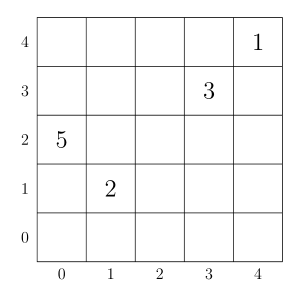
\includegraphics{fish-sample1-pond.png}   & 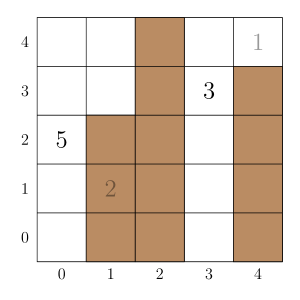
\includegraphics{fish-sample1-pier.png}\\
\hline
\end{tabular}
\end{center}

Число в клекте означает вес сома, расположенного в клетке.
Закрашенные клетки покрыты пирсами.
В это варианте сом $0$ (в клетке $(0, 2)$) и сом $3$ (в клетке $(3, 3)$) могут быть пойманы.
Сом $1$ (в клетке $(1, 1)$) не может быть пойман, так как его клетка покрыта пирсом, а сом $2$ (в клетке $(4, 4)$) не может быть пойман, так как нет пирса непосредственно к западу или к востоку от него.

Бу Денгклек хочет построить пирсы таким образом, чтобы суммарный вес сомов, которых можно поймать, был максимально возможным.
Ваша задача найти максимально возможный суммарный вес сомов, которых может поймать Бу Денгклек после постройки пирсов.


\textbf{Implementation Details}

Вы должны реализовать следующую функцию:

\begin{itemize}
    \item \texttt{int64 max\_weights(int N, int M, int[] X, int[] Y, int[] W)}
    \begin{itemize}
        \item $N$: размер водоёма.
        \item $M$: количество сомов.
        \item $X$, $Y$: массивы длины $M$, описывающие расположение сомов.
        \item $W$: массив длины $M$, описывающий веса сомов.
        \item Эта функция должна возвращать целое число, представляющее собой максимально возможный суммарный вес сомов, которых может поймать Бу Денгклек после постройки пирсов.
        \item Эта функция будет вызвана ровно один раз.
    \end{itemize}
\end{itemize}